\newpage
\subsection{Mechanical design}
\label{sec:method_mechanical}
This section shall describe the thought process and functionality of the mechanical part of the project.

\subsubsection{Idea}
The main constriction, the bulky 4x20 LCD, limits the compactness of the design. On the other hand, it simplifies the final product because there are limited options to include the display logically.

Right from the get-go, we decided that the switching between modes would not be done via a rotary switch, but rather digitally via a relay-matrix. This is important for mechanical design since it determines the functionality and what is needed to consider when designing the enclosure. By using the digitalized version of switching between modes, the only things we needed access to from the outside of the enclosure were:
% \newpage
\begin{itemize}
    \item Two buttons to control the modes (Next mode - previous mode)
    \item Reading the LCD
    \item Easy access to the 9V battery
    \item Being able to access the on/off switch
    \item Program the Arduino Nano
    \item Access to screws to disassemble the multi-meter
\end{itemize}
And with the exterior brainstormed, the interior needed some thinking. The requirements there would be:
\begin{itemize}
    \item An isolated place for the battery
    \item A way to fasten our PCB
    \item Somehow be able to access the buttons from the PCB
    \item The assembly screws to have threads to attach themselves
\end{itemize}
\label{sec:points}
\newpage
\subsubsection{Implementation}
With the points in \ref{sec:points} as a guide, the design would centre around the LCD. We decided that the best way to see the display from as many angles as possible, the LCD would need to be angled, in this case 30$^{\circ}$. \newline
The PCB will be mounted on the bottom of the case and the inner surface area will determine the cut-out of the PCB. This was done with the CAD-program Fusion 360 from Autodesk, a sketch-based CAD entity. This allows us to export the sketch we created, determining the dimensions of the PCB, to an .dxt-file which can be imported to KiCad 7.0, as a cut-out. By doing it like this, we can also direct where the mounting holes will be so that they will line up.
The sketch also considers the placement of both the 9V battery as well as the ON/OFF switch. This can be seen in Figure \ref{fig:sketchPCB}.
\begin{figure}[h]
    \centering
    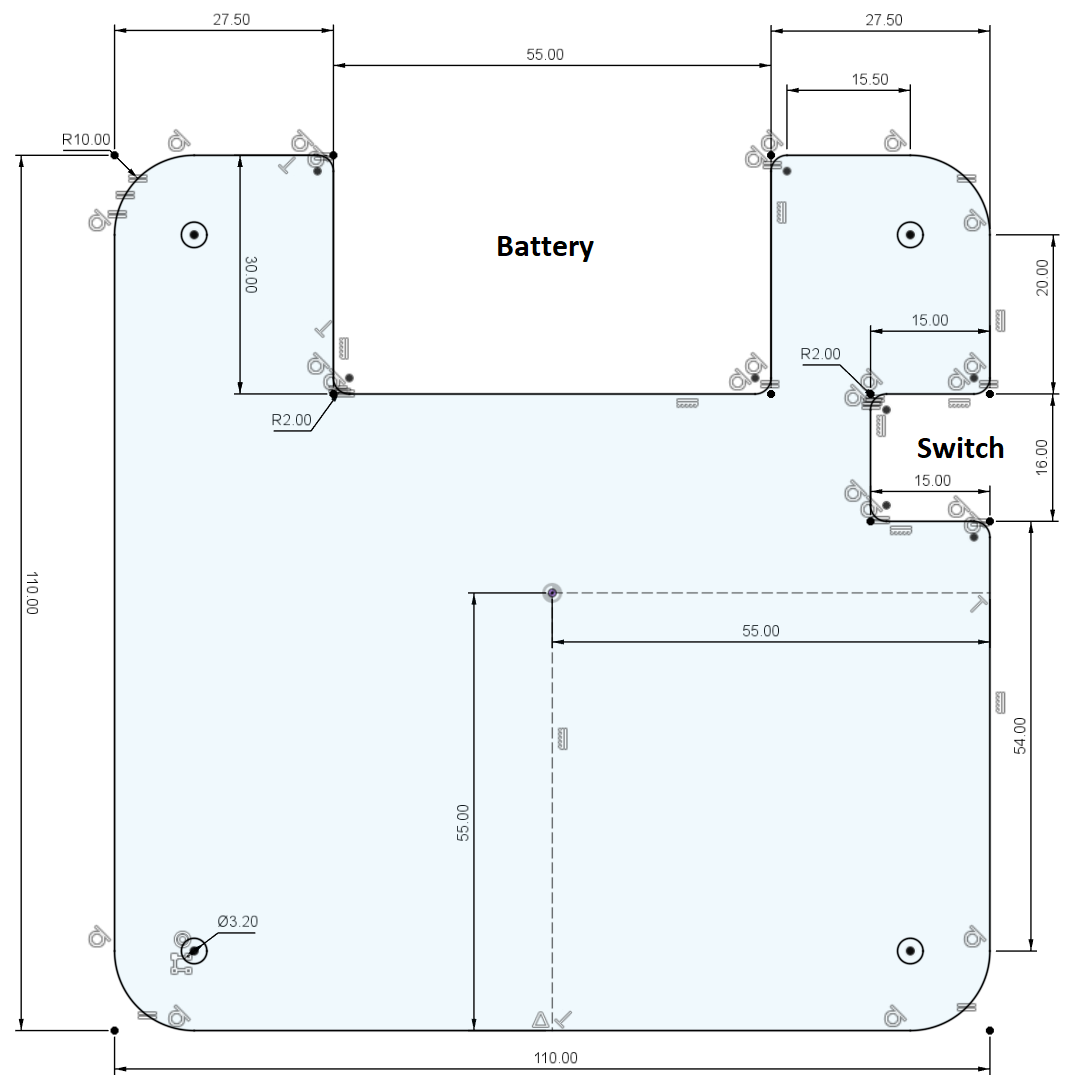
\includegraphics[width=\linewidth]{images/sketch-pcb-cutout.png}
    \caption{Final sketch of the PCB cut-out}
    \label{fig:sketchPCB}
\end{figure}
\newpage 
\noindent By importing various components to Fusion 360, it was also possible to place these components on the extruded PCB, to then help visualize how the next steps of the design process should proceed. Things like:
\begin{itemize}
    \item Placement of the two buttons needed for the menu switching
    \item Where the three 4mm banana plugs will stick out
    \item Placement of the Arduino Nano port
\end{itemize}
\begin{figure}[h]
    \centering
    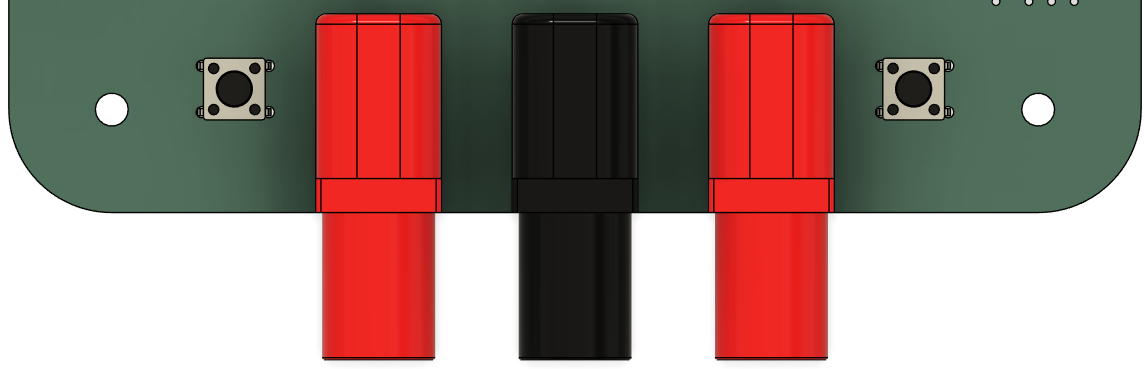
\includegraphics[width=\linewidth]{images/sketch-placement-plugsbut.png}
    \caption{Example of the placement of plugs and buttons}
    \label{fig:placeplugbut}
\end{figure}
Figure \ref{fig:placeplugbut} shows that the placement can easily be visualized. By then using measurements, the positioning of these components can be translated into the layout section of the PCB design in KiCad.
This comes with a trade-off, because the PCB is at the bottom of the case, the buttons would not be reachable. This problem is solved with what is called a 'button guide'. This was made with a 3D-printed cylinder which makes the buttons reachable from the outside.

This is shown in Figure \ref{fig:guide}.
\begin{figure}[h]
    \centering
    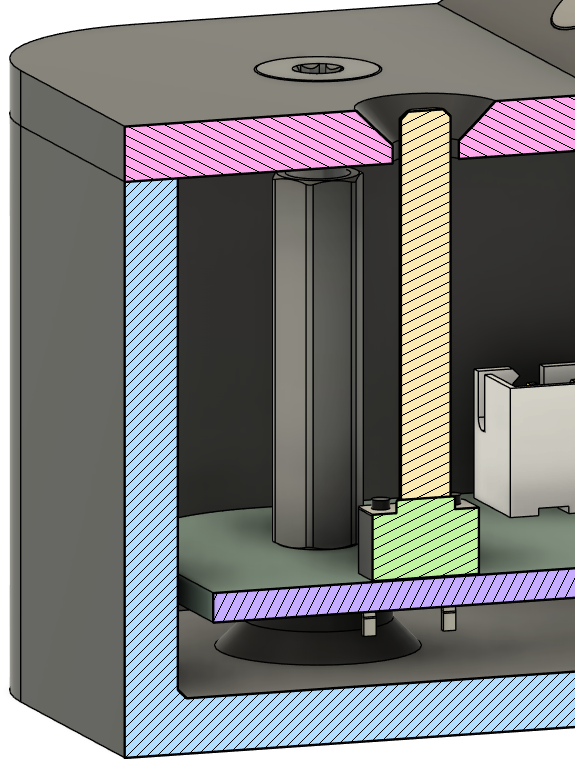
\includegraphics[width=0.35\linewidth]{images/guide.png}
    \caption{'Guide'-concept (\textcolor{GreenYellow}{yellow}), button (\textcolor{green}{green})}
    \label{fig:guide}
\end{figure}
\newpage
The mounting of the PCB to the bottom case was done via four extruded cylinders, where there was room enough to include M3 brass threaded inserts. These are inserted after the case is printed, with the tool soldering iron, set at 160$^\circ$-Celsius. This is illustrated in Figure \ref{fig:thread1}
\begin{figure}[h]
    \centering
    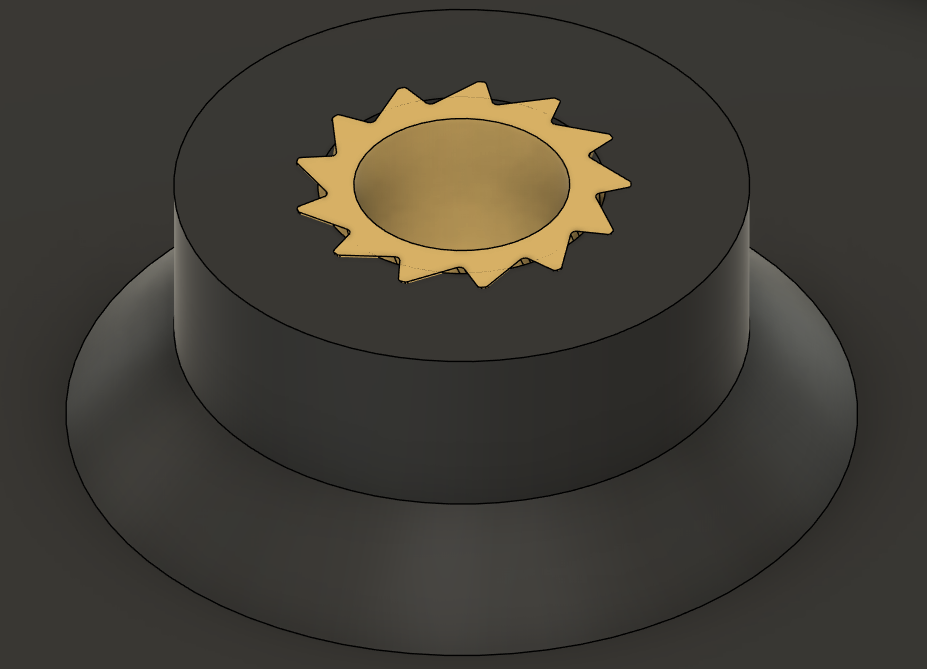
\includegraphics[width=0.5\linewidth]{images/threadinsert.png}
    \caption{Extruded cylinder w. threaded insert}
    \label{fig:thread1}
\end{figure}

We chose to have a no-tool hatch for easy access to the battery. With the combination of the 'battery low notification' via the LCD, it is then trouble-free to change the battery out in the field. This is seen in Figure \ref{fig:lid}.
\begin{figure}[h]
  \centering
  \subfloat[Without lid]{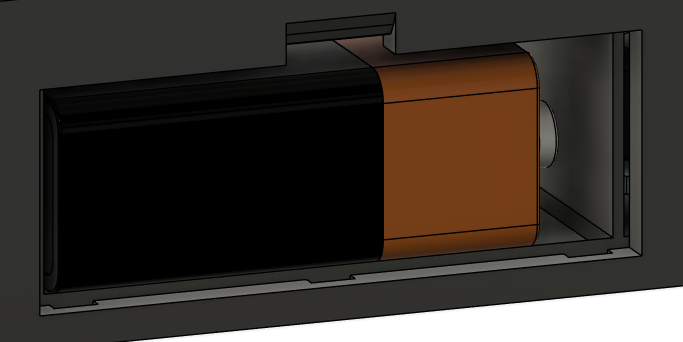
\includegraphics[width=0.4\textwidth]{images/batwolid.png}
  \label{fig:lida}}
  \hfill
  \subfloat[With lid]{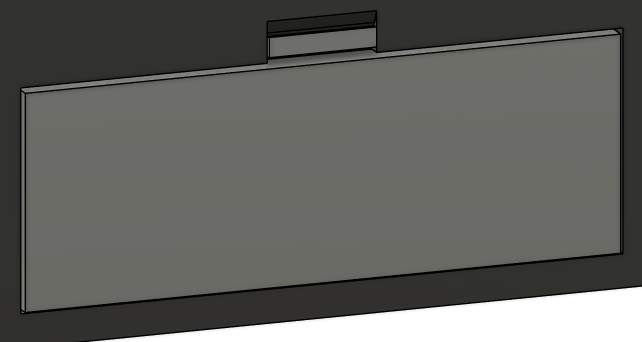
\includegraphics[width=0.375\textwidth]{images/batwlid.png}
  \label{fig:lidb}}
  \caption{Battery-lid placement}
  \label{fig:lid}
\end{figure}

To help isolate the battery, the bottom part of the case comes with a built-in 1mm wall separating the battery and the PCB. This is done for safety concerns since the possibility of short-circuiting is present. This is shown in Figure \ref{fig:batiso}.
\begin{figure}[h]
    \centering
    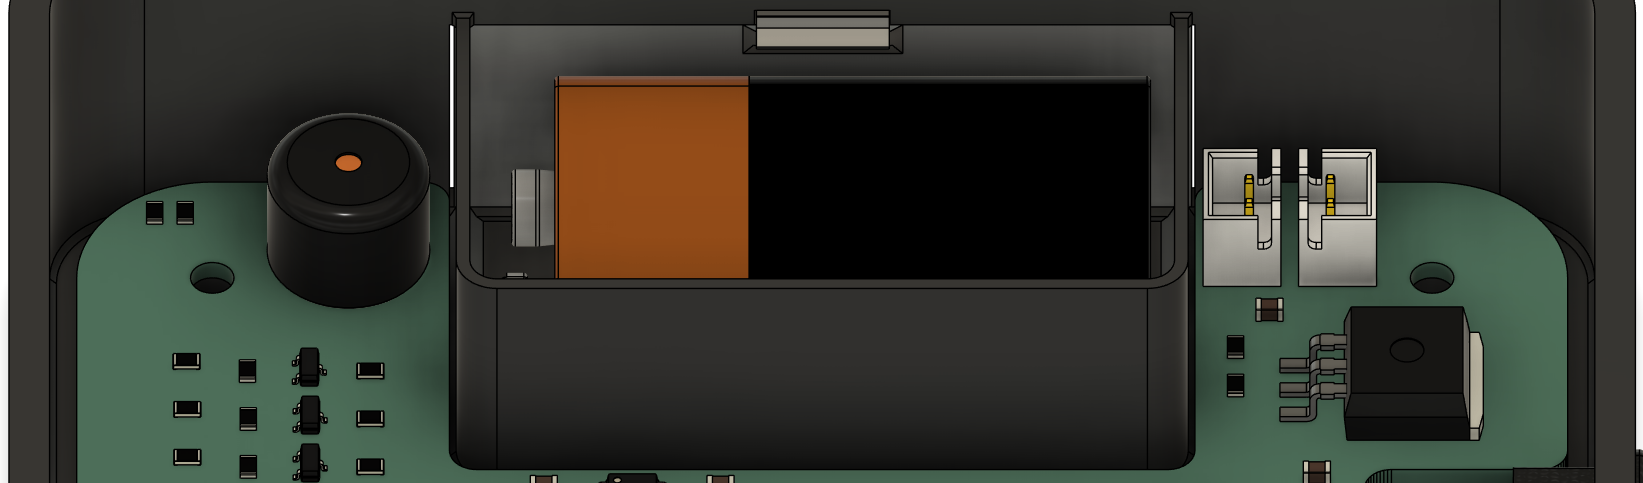
\includegraphics[width=0.855\linewidth]{images/batiso.png}
    \caption{Wall between PCB and battery}
    \label{fig:batiso}
\end{figure}
\newpage 
\noindent 
To then attach the upper part of the case, the lid w. the LCD, the method was to combine our threaded inserts and then attach PCB spacers at a length of 20mm. This is seen in Figure \ref{fig:guide} as the grey column with the screw attached.

\begin{figure}[h]
  \centering
  \subfloat[Without top]{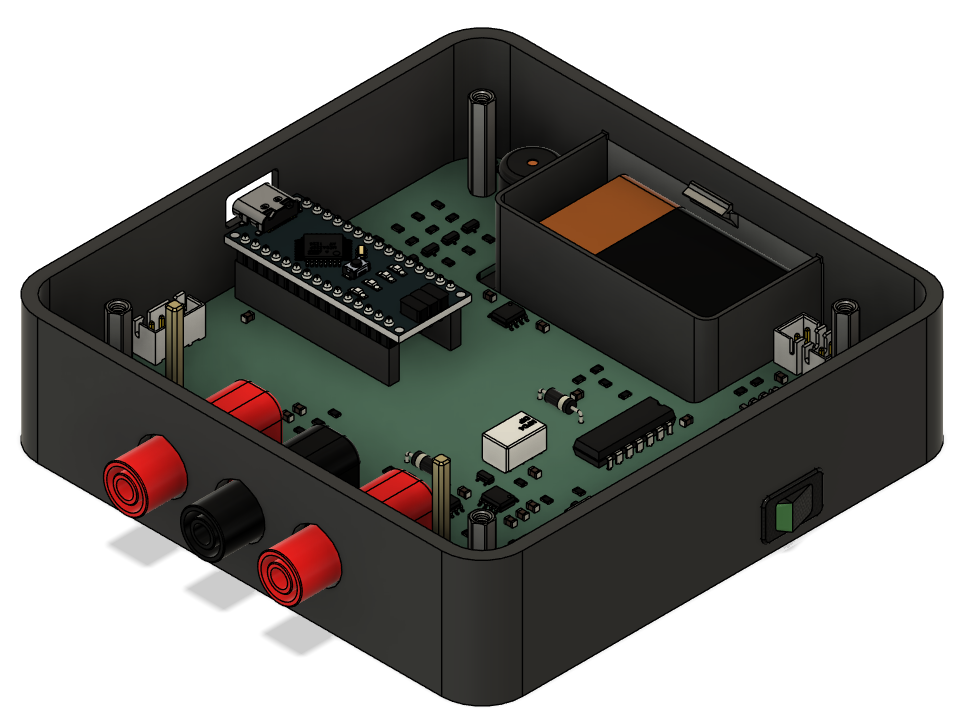
\includegraphics[width=0.65\textwidth]{images/bottom.png}
  \label{fig:enclA}}
  \hfill
  \subfloat[With top]{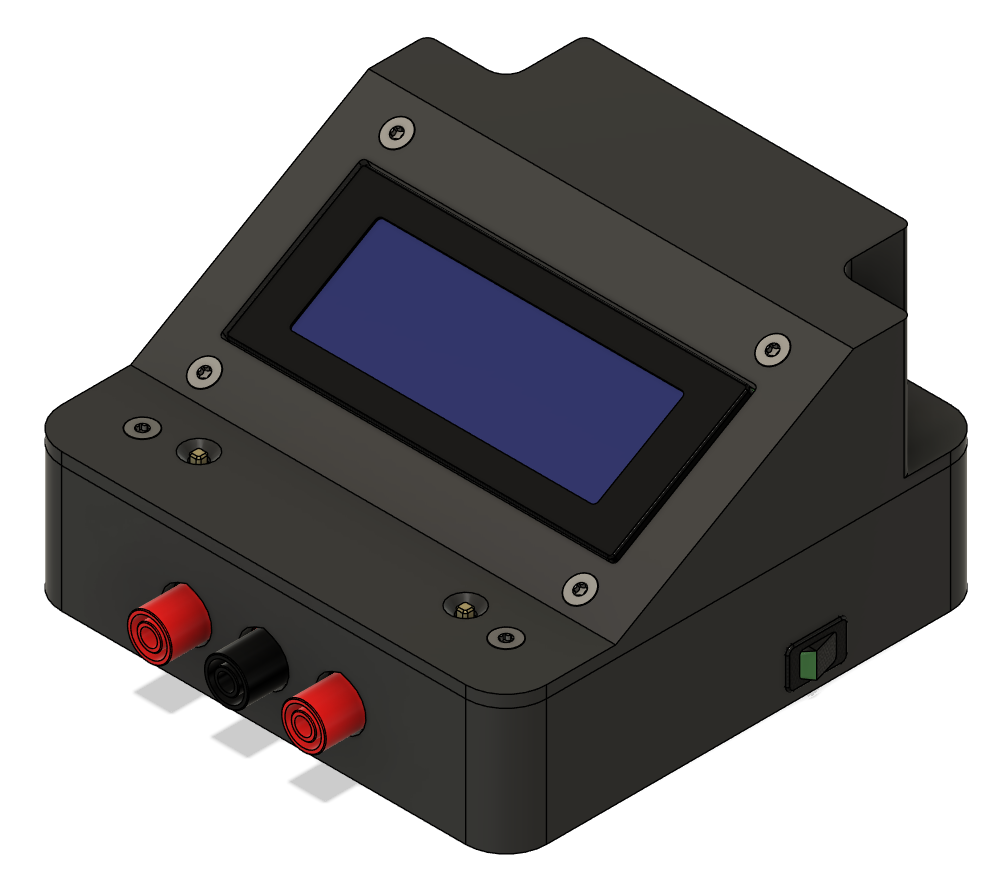
\includegraphics[width=0.65\textwidth]{images/total.png}
  \label{fig:enclB}}
  \caption{Final product}
  \label{fig:lid}
\end{figure}

\noindent The enclosure material is PLA+ and printed using a private Prusa MK3S+ FDM printer. See the Appendix for the top and bottom drawings of the enclosure.